% CAPITULO 1-------------------------------------------------------------------

\chapter{TAREFA 1}
\label{sec:qualidade}

\section{EAP}

A EAP (Estrutura Analítica do Projeto), do inglês \textit{Work Breakdown Structure} (WBS), é uma subdivisão hierárquica do trabalho do projeto em partes menores, mais facilmente gerenciáveis. Seu objetivo primário é organizar o que deve ser feito para produzir as entregas do projeto

A EAP garante ao gerente de projetos a visibilidade das principais entregas, facilitando o controle de tempo e de custo. Ela faz parte do processo de gerenciamento de escopo do projeto, descrito no Guia PMBOK® (\textit{Project Management Body of Knowledge}), uma das principais referências em gestão de projetos do mundo.

\section{Qual a diferença entre a EAP e o Cronograma?}

O cronograma de projeto é um instrumento de gestão, muitas vezes organizado em forma de quadro, que serve para controlar o tempo de um projeto. Com essa visão de cronograma, é possível identificar mais facilmente desvios que podem acontecer no projeto e, assim, tomar ações para corrigi-los. Portanto, o cronograma contém:


\begin{itemize}
\item Lista de atividades do projeto;
\item Data de início de cada atividade;
\item Data de término de cada atividade;
\item Responsável por cada atividade;
\item Status de cada atividade.
\end{itemize}

Diferentemente do cronograma, a estrutura analítica do projeto não comporta atividades. A sua última unidade de decomposição é o pacote de trabalho. Um pacote de trabalho, por sua vez, é um conjunto de atividades, normalmente atribuído a um departamento (que recebe orçamento para fazer uma entrega específica). Pacotes de trabalho devem ser independentes uns dos outros e não devem se repetir ao longo da estrutura analítica do projeto.

\section{Como fazer uma EAP (Estrutura Analítica do Projeto)}

Os padrões do PMI, seja o Guia PMBOK ou o Practice Standard for Work Breakdown Structures, refletem sempre as boas práticas utilizadas pelo mercado. Dessa forma, cabe ao gerente de projetos escolher a maneira de desdobrar a estrutura analítica do projeto junto com a equipe. A EAP pode ser mais orientada a produtos ou ao ciclo de vida do projeto, mas precisa ser útil tanto no planejamento quanto no monitoramento posterior.

Existem, basicamente, quatro estratégias para montar a EAP:

\begin{itemize}
\item Por fases: considera as fases do ciclo de vida do projeto.
\item Por entregas: considera os produtos do projeto.
\item Por subprojeto: considera os “miniprojetos” que compõem o projeto;
\item Híbrida (por fases, entregas e/ou subprojetos): considera diversos aspectos do projeto ao mesmo tempo.
\end{itemize}

\section{Exemplo de EAP (Estrutura Analítica do Projeto)}

Vamos imaginar que nosso projeto é construir uma casa e que optamos por uma estratégia de decomposição híbrida, com fases e entregas. Utilizando os três níveis e o sistema de codificação numérico temos a seguinte estrutura analítica de projeto:

\begin{figure}[H]
    \centering
    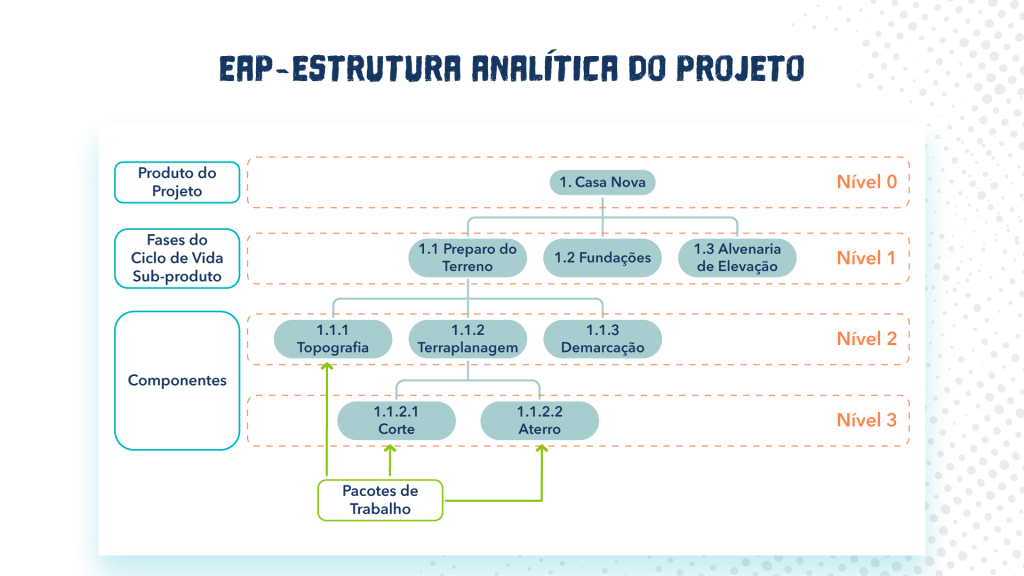
\includegraphics[width=0.7\linewidth]{dados/figuras/eap}
    \caption{EAP - Estrutura Analítica}
    \label{fig:eap}
\end{figure}

\section{Modelo de EAP}

Quando se trabalha com frequência num mesmo tipo de projeto, é possível evoluir a EAP e transformá-la num modelo. Isso tornará novos projetos muito mais rápidos, pois teremos um modelo de estrutura analítica de projeto, de cronograma, de estimativa de recursos e durações, tudo padronizado, algumas etapas economizadas, bastando uma adequação e revisão a cada projeto.

\section{Como montar o Dicionário da EAP (Estrutura Analítica do Projeto)}

O dicionário da EAP é uma tabela que descreve os pacotes de trabalho, seus responsáveis e critérios de aceitação. Essa ferramenta ajuda a complementar a estrutura analítica do projeto, pois traz informações que não puderam ser incluídas no diagrama da EAP. Dessa forma, ficam explícitas quais as expectativas em relação aos resultados das entregas do projeto.

Voltando ao nosso exemplo da casa, poderíamos ter o seguinte “verbete” no dicionário da EAP:

\begin{itemize}
\item Pacote de Trabalho: alvenaria de elevação
\item Descrição: levantamento de paredes, utilizando o método especificado no projeto de construção civil.
\item Responsável: Pedro Alcântara.
\item Participantes: Flávia Marcelino, Kássio Freitas.
\item Critérios de Aceitação: firmeza, ausência de rachaduras, bom isolamento térmico.
\end{itemize}

O dicionário da EAP é ótimo para ser consultado quando alguém fica com dúvidas a respeito daquilo que deve ser entregue, facilitando a comunicação do time. Além disso, também auxilia na hora de construir o cronograma, segundo passo depois da elaboração da EAP.
\nocite{eap}
